\documentclass[10pt,letterpaper, onecolumn]{report}
\usepackage{amsmath}
\usepackage{amssymb}
\usepackage{listings}
\usepackage{xcolor}
\usepackage[lmargin=71pt, tmargin=0.6in]{geometry}  % For centering solution box
\usepackage{fancyhdr}
\usepackage{graphicx}

% Define the footer format
\pagestyle{fancy}

% Clear any existing footer content
\fancyhead{}
\fancyfoot{}

% Set footer contents: center text and page number on the right
\fancyfoot[L]{Author: Kacper Ragankiewicz, Index: 283415 } % Centered footer
\fancyfoot[R]{\thepage} % Right-aligned page number

% Define colors similar to VS Code's Python syntax
\definecolor{keywordcolor}{rgb}{0.58, 0.01, 0.24}   % Red for keywords
\definecolor{stringcolor}{rgb}{0.44, 0.55, 0.34}    % Green for strings
\definecolor{commentcolor}{rgb}{0.5, 0.5, 0.5}      % Gray for comments
\definecolor{backgroundcolor}{rgb}{0.97, 0.97, 0.97} % Light gray background

\lstdefinestyle{myPythonStyle}{
    language=Python,
    backgroundcolor=\color{backgroundcolor},    % Set background color
    basicstyle=\ttfamily\small,                 % Monospaced font with small size
    keywordstyle=\color{keywordcolor}\bfseries,  % Red for keywords (bold)
    stringstyle=\color{stringcolor},             % Green for strings
    commentstyle=\color{commentcolor}\itshape,   % Gray and italic for comments
    numberstyle=\tiny\color{gray},               % Line numbers in gray
    numbersep=5pt,                              % Space between line numbers and code
    stepnumber=1,                               % Number every line
    numbers=left,                               % Place line numbers to the left
    showstringspaces=false,                     % Don't show space characters
    tabsize=4,                                  % Set tab size
    breaklines=true,                            % Automatically break long lines
    frame=single,                               % Draw a frame around the code block
    rulecolor=\color{black},                    % Color for the frame
}

\renewcommand{\headrulewidth}{0pt}

\begin{document}

% Title and other front matter
\begingroup
    \centering
    \LARGE \textbf{Complex Systems} \\
    \large CS2024/problem\_3.pdf \\[0.5em]
\endgroup

\begin{flushleft}
    \rule{\textwidth}{0.4pt} \\ % Horizontal line
    \textbf{Result} % Text aligned to the left
\end{flushleft}

\begin{flushleft}
    \textbf{3 Self-organized criticality: the Oslo model}
    \hfill\break
    \setlength{\parindent}{1.5em} % Adjust paragraph indentation
    \setlength{\parskip}{0.5em}   % Adjust paragraph spacing

    The Oslo rice-pile model is a theoretical model of self-organized criticality (SOC) used to study
    the behavior of granular materials and avalanche-like phenomena in a simple, discrete system. It was
    introduced as a variation of the sandpile model, and it's named after the city of Oslo, Norway, where it
    was developed.
\end{flushleft}

\begin{flushleft}
    \begin{enumerate}
        \item Implement the Oslo model using the following algorithm focusing on slopes $z_{i}$ :
        \begin{enumerate}
            \item Initialize the system in arbitrary stable configuration $z_{i} \leqslant z_{t}^T$, where $z_{i}^T$ is i-th slope threshold $ \in \left\{ 1,2 \right\}$;
            \item Drive the system by adding a grain at left-most site;
            \item If $z_{i} < z_{i}^T$, relax the site i,
            \begin{itemize}
                \item[] for $i=1: z_{1} \to z_{1} - 2, z_{2} \to z_{2} + 1$;
                \item[] for $i=2 \dots L-1: z_{i} = z_{i} - 2, z_{i \pm 1} \to z_{i \pm 1} + 1$;
                \item[] for $i=L: z_{L} \to z_{L} - 1, z_{L-1} \to z_{L-1} + 1$;
            \end{itemize}
            During relaxation do not forget about choosing randomly new threshold $z_{t}^T i \in \left\{ 1,2 \right\}$ for the relaxed site. Continue relaxation until $ z_{i} \leqslant z_{i}^T$ for all $i$;
            \item Return to point (b).
            \hfill\break
            \begin{lstlisting}[style=myPythonStyle, caption={Oslo Model Algorithm (Python version 3.11.7)}]
import numpy as np
import matplotlib.pyplot as plt

def oslo_model(L, T, z_thresholds=[1, 2]):
    """
    Simulates the Oslo model of self-organized criticality.

    Parameters:
    - L: int, size of the system (number of sites).
    - T: int, number of grain additions (time steps).
    - z_thresholds: list, possible slope thresholds (default is [1, 2]).

    Returns:
    - avalanches: list, size of avalanches during the simulation.
    """

    slopes = np.random.choice(z_thresholds, size=L)  # (a) Initial random slopes in {1, 2}
    thresholds = np.random.choice(z_thresholds, size=L) # (a) Initial random thresholds in {1, 2}
    avalanches = []

    for t in range(T):
        slopes[0] += 1 # (b) Add a grain to the left-most site
        avalanche_size = 0

        # (c) Relaxation process
        while np.any(slopes > thresholds):
            for i in range(L):
                if slopes[i] > thresholds[i]:
                    avalanche_size += 1
                    thresholds[i] = np.random.choice(z_thresholds)  # Assign a new threshold

                    if i == 0:  # Left-most site
                        slopes[i] -= 2
                        slopes[i + 1] += 1
                    elif i == L - 1:  # Right-most site
                        slopes[i] -= 1
                        slopes[i - 1] += 1
                    else:  # Internal sites
                        slopes[i] -= 2
                        slopes[i - 1] += 1
                        slopes[i + 1] += 1

        avalanches.append(avalanche_size)

    return avalanches
            \end{lstlisting}
        \end{enumerate}
        \hfill\break

            \item Plot scaled avalanche size $ s/s_{max} $ in function of time $t$ (measured in terms of grain additions). Does
            it make sense to analyze data for small $t$? Which condition should be satisfied in avalanche size
            statistical analysis?
            \hfill\break


            \begin{lstlisting}[style=myPythonStyle, caption={Oslo Model Algorithm (Python version 3.11.7)}]
L = 2  # System length
T = 4  # Number of time steps
avalanches = oslo_model(L, T)

# Scaled avalanche sizes
s_max = max(avalanches)
scaled_avalanches = [s / s_max for s in avalanches]

# Plotting
plt.figure(figsize=(10, 6))
plt.plot(range(T), scaled_avalanches, label='Scaled Avalanche Size')
plt.xlabel('Time (Grain Additions)')
plt.ylabel('Scaled Avalanche Size $s/s_{max}$')
plt.title('Scaled Avalanche Size vs. Time')
plt.grid(True)
plt.legend()
plt.savefig('avalanche_one.png')
plt.show()
            \end{lstlisting}
            \clearpage

            \begin{figure}[htbp!]
                \centering
                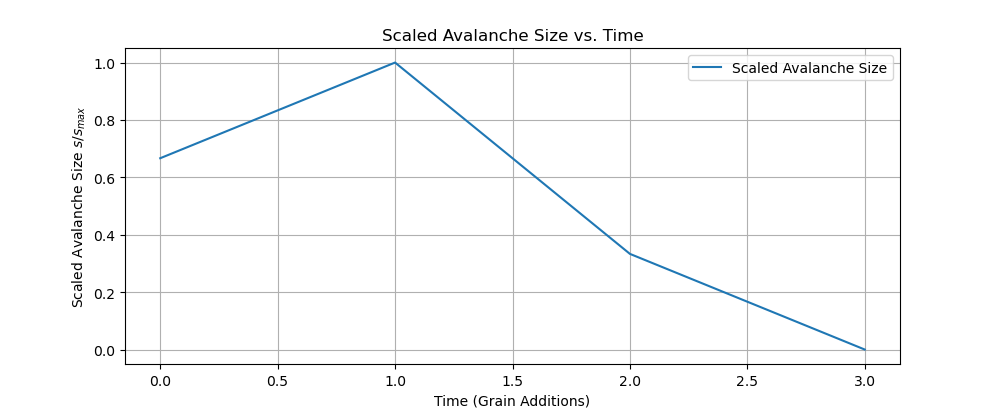
\includegraphics[width=0.9\textwidth]{../avalanche_one.png}
                \caption{Plot for L = 2, T = 4}
            \end{figure}

            \begin{figure}[htbp!]
                \centering
                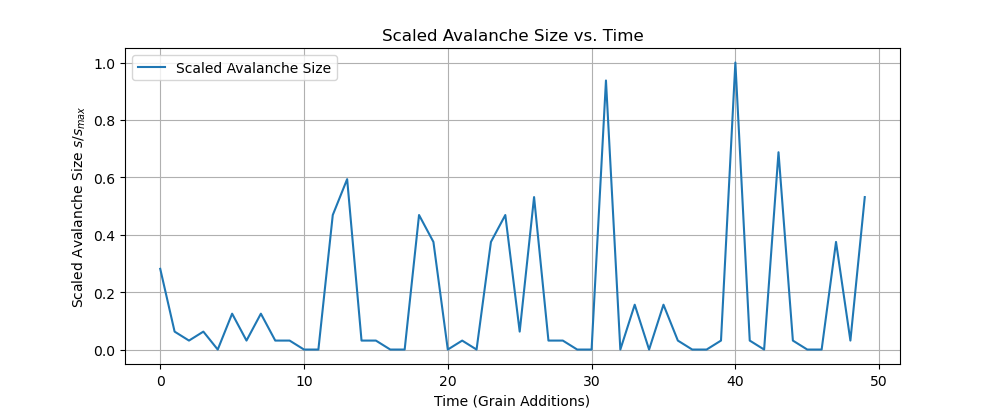
\includegraphics[width=0.9\textwidth]{../avalanche_small.png}
                \caption{Plot for L = 6, T = 50}
            \end{figure}

            \begin{figure}[htbp!]
                \centering
                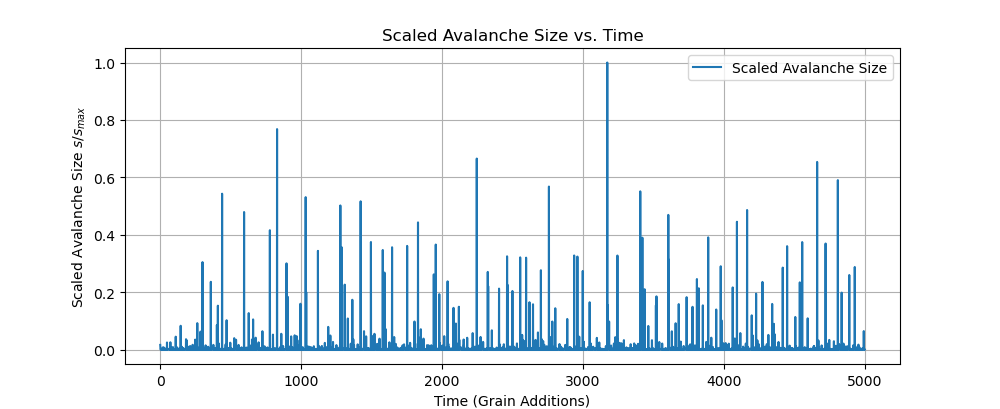
\includegraphics[width=0.9\textwidth]{../avalanche_big.png}
                \caption{Plot for L = 64, T = 5000}
            \end{figure}

            \clearpage

            Does it makes sense to analyze data for small $t$?
            \hfill\break

            \hspace{1.5em}\textbf{ANSWER:} It doesn’t make sense to analyze data for small t because the system has not reached its critical state yet, and the results will not be representative of the true behavior of the system.
            \hfill\break

            What condition should be satisfied in avalanche size statistical analysis?
            \hfill\break

            \hspace{1.5em}\textbf{ANSWER:} The system should be in steady state, and you need a large number of grains added to the system for meaningful results (to observe the power-law distribution of avalanche sizes).

            \hfill\break
            \item Plot in log-log scale avalanche size probability $P (s, L)$ with respect to avalanche size $s$ for several
            lengths of the system ($L$ should be at least 64). Do you observe power law behavior? Why does this
            power law break for large $s$?
            \hfill\break
            \begin{lstlisting}[style=myPythonStyle, caption={Oslo Model Algorithm (Python version 3.11.7)}]
from scipy.stats import linregress
import numpy as np
import matplotlib.pyplot as plt


def avalanche_probability(avalanches, L_values, name, min_s=1, max_s=200):
    """
    Plot avalanche size probability P(s, L) in log-log scale with points and linear regression.

    Parameters:
    - avalanches: list of lists, avalanches for different system lengths.
    - L_values: list of int, system lengths.
    - name: str, name for the saved plot file.
    - min_s: float, minimum avalanche size for fitting the power-law.
    - max_s: float, maximum avalanche size for fitting the power-law.
    """
    plt.figure(figsize=(10, height))

    for avals, L in zip(avalanches, L_values):
        if len(avals) == 0:
            print(f"No data for L={L}, skipping.")
            continue

        # Remove non-positive values
        avals = np.array([a for a in avals if a > 0])

        if len(avals) == 0:
            print(f"All data for L={L} are zero or invalid, skipping.")
            continue

        # Calculate probabilities
        avalanche_sizes, counts = np.unique(avals, return_counts=True)
        probabilities = counts / sum(counts)

        # Plot points
        plt.scatter(avalanche_sizes, probabilities, label=f'L={L}', alpha=0.7)

        # Filter for power-law range
        valid_range = (avalanche_sizes >= min_s) & (avalanche_sizes <= max_s)
        filtered_sizes = avalanche_sizes[valid_range]
        filtered_probs = probabilities[valid_range]

        if len(filtered_sizes) > 1:  # Fit only if sufficient data
            # Linear regression in log-log space
            log_sizes = np.log10(filtered_sizes)
            log_probs = np.log10(filtered_probs)
            slope, intercept, _, _, _ = linregress(log_sizes, log_probs)

            # Calculate the fitted regression line in log-log space
            regression_line = slope * log_sizes + intercept

            # Convert back to the original scale for plotting
            fitted_probs = 10 ** regression_line

            # Plot regression line
            plt.plot(filtered_sizes, fitted_probs, label=f'L={L} (Exponent={-slope:.2f})', linestyle='--')

            # Print exponent for verification
            print(f"L={L}: Slope = {slope:.4f}, Exponent = {-slope:.4f}")

    # Configure log-log scale
    plt.xscale('log')
    plt.yscale('log')
    plt.xlabel('Avalanche Size $s$')
    plt.ylabel('Probability $P(s, L)$')
    plt.title('Avalanche Size Probability $P(s, L)$ in Log-Log Scale')
    plt.legend()
    plt.grid(True, which='both', ls='--')

    # Save the plot
    plt.savefig(f'probability_{name}.png')
    plt.show()

L = 6
T = 50

# Simulations for different system sizes
L_values = [64, 128, 256]
avalanche_data = [oslo_model(L, T) for L in L_values]

# Compute and plot probabilities
avalanche_probability(avalanche_data, L_values, 'one')
            \end{lstlisting}
            \clearpage

            \begin{figure}[htbp!] % Positioning options: here, top, bottom, page
                \centering
                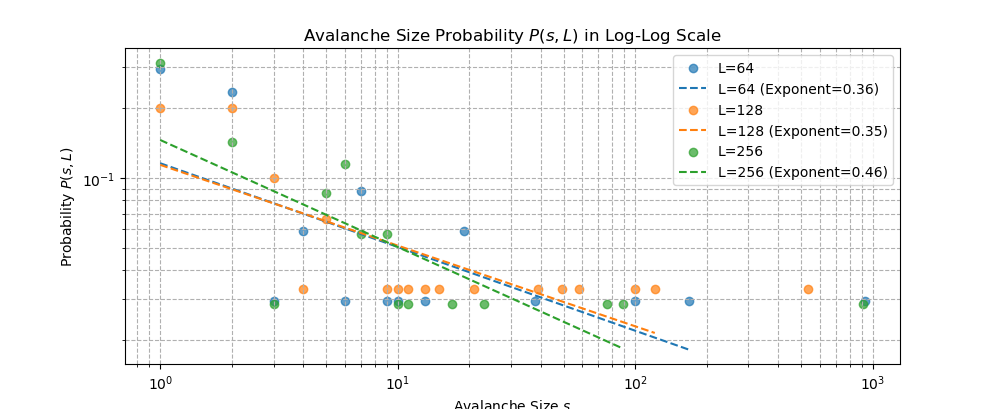
\includegraphics[width=0.9\textwidth]{../probability_one.png} % Specify image file and scale
                \caption{Plot for $L = 6$, $T = 50$, and $L \in \{64, 128, 256\}(0.4s)$} % Caption for the image
            \end{figure}
            \begin{figure}[htbp!] % Positioning options: here, top, bottom, page
                \centering
                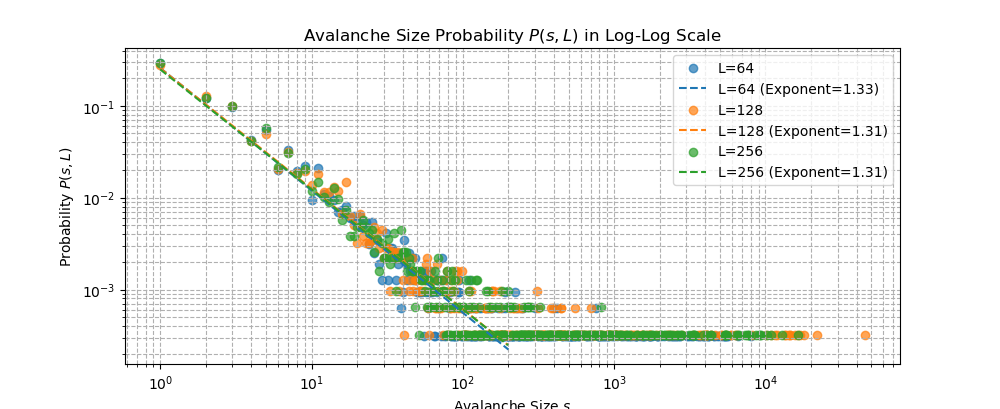
\includegraphics[width=0.9\textwidth]{../probability_small.png} % Specify image file and scale
                \caption{Plot for $L = 64$, $T = 5000$, and $L \in \{64, 128, 256\}(6.8s)$ } % Caption for the image
            \end{figure}
            \begin{figure}[htbp!] % Positioning options: here, top, bottom, page
                \centering
                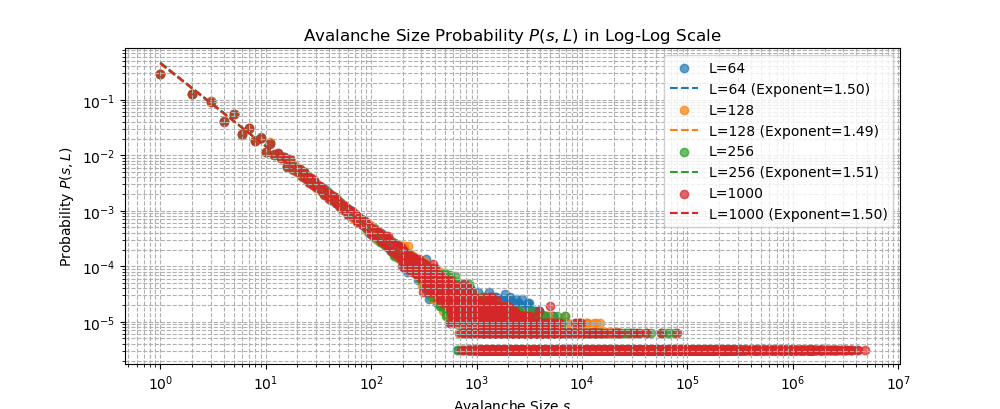
\includegraphics[width=0.9\textwidth]{../probability_big_long.png} % Specify image file and scale
                \caption{Plot for $L = 64$, $T = 500000$, and $L \in \{64, 128, 256, 1000\}(54m 58.9s)$} % Caption for the image
            \end{figure}

            \clearpage

            Do you observe power law behavior in the avalanche size distribution?
            \hfill\break

            \hspace{1.5em}\textbf{ANSWER:} Yes, I observe a power law behavior in the avalanche size distribution for the Oslo model, once the system has reached self-organized criticality (SOC).
            \hfill\break

            Why does this power law break for large $s$?
            \hfill\break

            \hspace{1.5em}\textbf{ANSWER:} The power law breaks down for large s because of finite system size (limited number of sites), saturation of the system, statistical sampling limitations, and time constraints. The probability of very large avalanches is reduced, leading to a cutoff in the distribution.

            \hfill\break
        \end{enumerate}
        \end{flushleft}
\end{document}
